\header{
    \section{En revenant du Piémont} \label{en-revenant-du-piemont}
    %
    
    \insertComment{Chanson sur les guerres d'Italie imprimée en 1530.}{}
}

\enluminure{4}{\href{https://www.youtube.com/watch?v=QTRL4ILGLBo}{E}}{n nous revenant} du Piémont,~~~~~~~~~~~~~~~~~\bissimple
\\Nous étions trois jeunes garçons,  ~~~~~~~~~~~~~~~\bissimple
\\Mais de l'argent nous n'en avions guère,
\\Sens dessus dessous et sens devant derrière.
\\A nous trois, nous n'avions qu'un sou,
\\Sens devant derrière et sens dessus dessous. ~~~~~~~~~~~~~~~~~~~\bissimple
\\\\Hôtesse, nous voulons manger,~~~~~~~~~~~~~~~~~\bissimple
\\Qu'avez-vous donc à nous donner ?  ~~~~~~~~~~  \bissimple
\\- J'ai du lapin, du civet de lièvre,
\\Sens dessus dessous et sens devant derrière.
\\Et de la bonne soupe aux choux,
\\Sens devant derrière et sens dessus dessous. \bissimple
\\\\Hôtesse, nous voulons coucher,~~~~~~~~~~~~~~~\bissimple
\\Qu'avez-vous donc à nous donner ?~~~~~~~~~~~~\bissimple
\\- J'ai ma chambre sur le derrière,
\\Sens dessus dessous et sens devant derrière.
\\Et ma servante qui couche en d'ssous,
\\Sens devant derrière et sens dessus dessous. \bissimple
\\\\Sur les onze heures, on entendit,~~~~~~~~~~~~~~~\bissimple
\\L'hôtesse pousser un grand cri. ~~~~~~~~~~~~~~~~\bissimple
\\- Ah! Vous me pétez la charnière,
\\Sens dessus dessous et sens devant derrière.
\\Allez-y donc un peu plus mou !
\\Sens devant derrière et sens dessus dessous. \bissimple
\\\\Mais quand ce fut sur les minuit ~~~~~~~~~~~~~~~\bissimple
\\Il se fit un bien plus grand bruit. ~~~~~~~~~~~~~\bissimple
\\C'était le lit du d'ssous qui s'fichait par terre,
\\Sens dessus dessous et sens devant derrière,
\\Et la servante qui baisait d'ssous,
\\Sens devant derrière et sens dessus dessous. ~ \bissimple
\breakpage
Quand vous repass'rez par ici, ~~~~~~~~~~~~~~~~\bissimple
\\Souvenez-vous du bon logis, ~~~~~~~~~~~~~~~\bissimple
\\Souvenez-vous d'la bonne hôtesse,
\\Qui remue le cul, sans remuer les fesses,
\\Et d'la p'tite bonne qui remue tout,
\\Sens devant derrière et sens dessus dessous. \bissimple
\\
\bigskip
\begin{center}
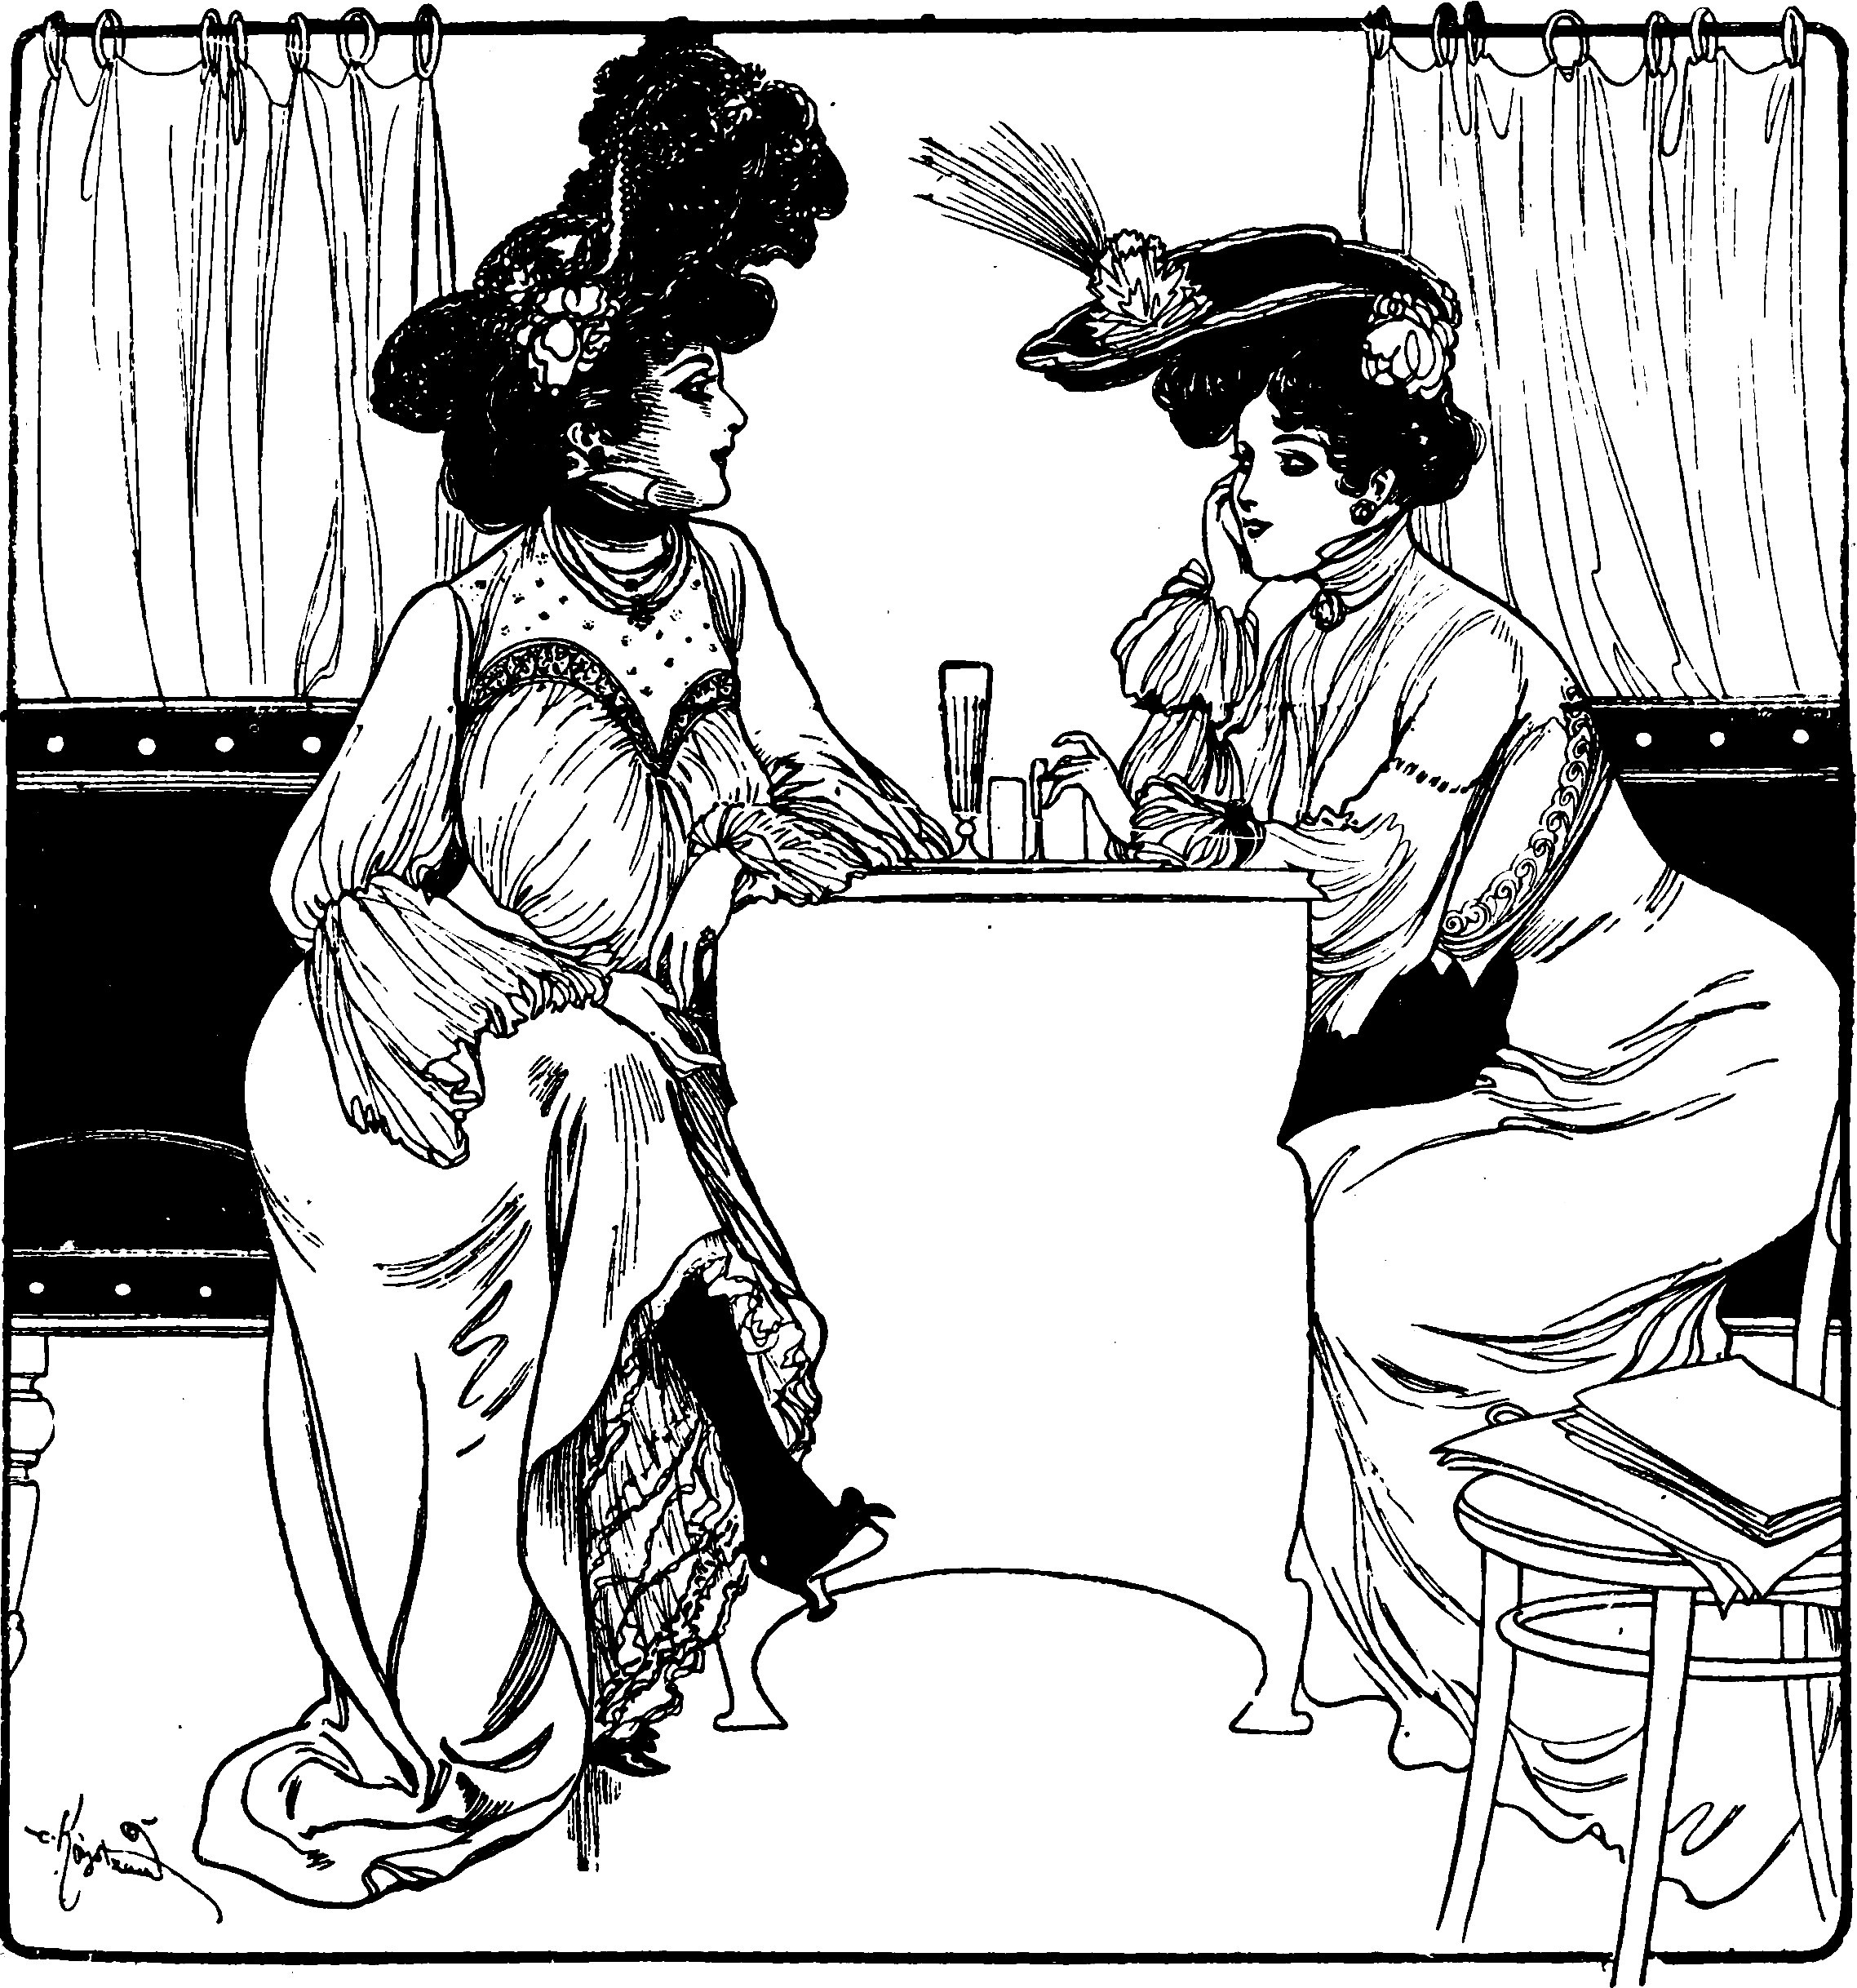
\includegraphics[width=1\textwidth]{images/brev3.png}
\end{center}

\breakpage